\documentclass[11pt]{article}
\usepackage[final]{acl}
\usepackage{times}
\usepackage{latexsym}
\usepackage[T1]{fontenc}
\usepackage[utf8]{inputenc}
\usepackage{microtype}
\usepackage{inconsolata}
\usepackage{graphicx}
\usepackage{amsmath}
\usepackage{amssymb}
\usepackage{booktabs}
\usepackage{multirow}
\usepackage{xspace}

\newcommand{\model}{GACA-BiGRU\xspace}
\title{Goal-Aware Contrastive Attention for Physical Commonsense Question Answering}
\author{Group GROUP\_ID}

\begin{document}
\maketitle

\begin{abstract}
We study PIQA, where a system selects the more physically plausible of two solutions to a natural-language goal. We introduce \model, a 1.33M-parameter model trained entirely from scratch. A shared bidirectional GRU encodes the goal and candidates; goal-conditioned additive attention extracts candidate evidence; and a swap-equivariant contrastive scorer directly compares the alternatives. On the held-out test set, \model obtains $60.65\pm0.33$ accuracy and $60.64\pm0.33$ macro-F1 over three seeds, exceeding majority, TF--IDF, and mean-pooled BiGRU baselines. Controlled ablations identify pairwise contrast as the largest contributor. Attention visualisations show useful lexical focus but also expose confident errors requiring unstated chemical or physical knowledge.
\end{abstract}

\section{Introduction}
Physical commonsense connects language to object affordances, materials, and causal consequences. Such facts are often omitted from text because people assume them, creating the reporting-bias challenge highlighted by \citet{bisk2020piqa}. PIQA operationalises this problem as two-choice question answering: given a goal such as ``protect a car from scratches,'' select the more sensible solution. Its deliberately similar alternatives reduce the value of topic matching and make relational comparison important.

Our aim is not to import knowledge through pretraining, but to test how far a compact task-specific architecture can learn from the supplied data alone. We propose \textbf{G}oal-\textbf{A}ware \textbf{C}ontrastive \textbf{A}ttention with a \textbf{BiGRU} (\model). It combines GRU sequence modelling \citep{cho2014gru}, additive attention \citep{bahdanau2015attention}, explicit goal--solution interactions, and a symmetric candidate comparison. Our contributions are: (1) a from-scratch, choice-order-equivariant PIQA model; (2) comparison with lexical and neural baselines plus controlled component ablations; and (3) quantitative and qualitative analysis over three main-model seeds. We find a modest but reproducible advantage, while error analysis shows that attention cannot supply physical knowledge absent from the training signal.

\section{Methodology}
Figure~\ref{fig:architecture} summarises the architecture. All embeddings and weights are learned from random initialisation; no pretrained representations or external data are used.

\subsection{Shared sequence encoder}
Let the tokenised goal be $G$ and alternatives $S_1,S_2$. A shared embedding matrix $E\in\mathbb{R}^{|V|\times d_e}$ and bidirectional GRU encode every sequence:
\begin{equation}
 H^x=\mathrm{BiGRU}(E(x)), \quad x\in\{G,S_1,S_2\}.
\end{equation}
Sharing prevents candidate-position-specific encoders. The goal vector $g$ is the padding-masked mean of $H^G$.

\subsection{Goal-conditioned attention}
For candidate $i$, additive attention scores each contextual state $h^i_t$ against the goal:
\begin{align}
 e_{it}&=v^\top\tanh(W_s h^i_t+W_g g),\\
 \alpha_{it}&=\mathrm{softmax}_{t}(e_{it}),\qquad
 a_i=\sum_t\alpha_{it}h^i_t .
\end{align}
Padding positions are masked before the softmax. Unlike unconditional pooling, this adapts candidate evidence to the requested goal. The design is adapted from additive alignment \citep{bahdanau2015attention} and query-aware reading \citep{seo2017bidaf}; our use here separately aligns each PIQA alternative to the same goal.

We form an interaction-rich candidate representation
\begin{equation}
 r_i=[g;a_i;g\odot a_i;|g-a_i|],
\end{equation}
where product and absolute difference expose soft agreement and mismatch to the scorer.

\subsection{Contrastive, swap-equivariant scoring}
PIQA alternatives are defined relationally, so scoring each in isolation wastes the competing evidence. For $j\neq i$ we construct
\begin{equation}
 z_i=[r_i;r_i-r_j;r_i\odot r_j], \quad \ell_i=f_\theta(z_i),
\end{equation}
where $f_\theta$ is a shared two-layer MLP. The prediction is $p(y=i)=\mathrm{softmax}(\ell_1,\ell_2)_i$. Swapping $S_1,S_2$ exactly swaps the two logits: the model cannot learn an answer-position shortcut. This paired contrast and its equivariance are our principal task-specific design contribution.

\begin{figure*}[t]
  \centering
  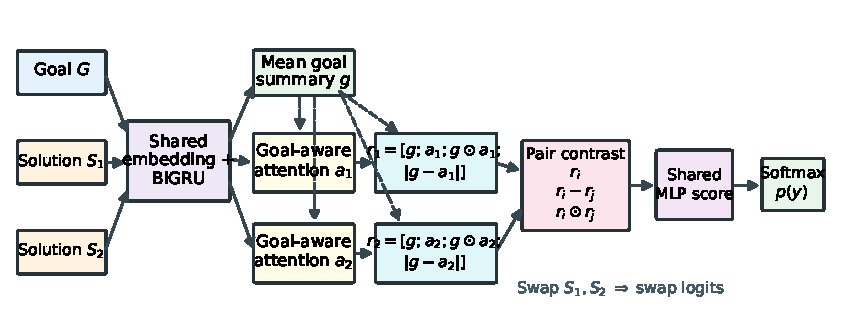
\includegraphics[width=0.98\textwidth]{architecture.pdf}
  \caption{\model. Dashed arrows carry the goal summary. The encoder and scorer are shared across candidate positions.}
  \label{fig:architecture}
\end{figure*}

\section{Experimental Setup}
\subsection{Data and preprocessing}
We use only the supplied PIQA files. The provided training set has 16,113 examples and the held-out test set 1,838. We create one fixed, stratified 85/15 split of the former (seed 2026): 13,696 training and 2,417 validation examples. Label 1 proportions are 50.02\%, 50.02\%, and 50.49\% respectively. The test set is excluded from model selection.

Text is lower-cased and tokenised with a deterministic regular expression retaining words, numbers, apostrophes, and punctuation. The vocabulary is built on training text only, retains tokens occurring at least twice, and contains 10,812 entries including padding and unknown symbols. Goals and solutions are truncated to 48 and 64 tokens; the solution 95th percentile is 61 tokens (maximum 472), so truncation affects fewer than 5\% of candidates.

\subsection{Training and reproducibility}
Embeddings have 96 dimensions; each GRU direction has 64 hidden units. The scorer has 128 hidden units with ReLU and dropout 0.25 \citep{srivastava2014dropout}. We train with cross-entropy, AdamW \citep{loshchilov2019adamw} (learning rate $2\!\times\!10^{-3}$, weight decay $10^{-4}$), batch size 256, and gradient-norm clipping at 5. Training runs for at most six epochs with validation-accuracy early stopping (patience two). These compact settings were chosen before final test evaluation to suit scratch training and Colab reproducibility. The main model is run with seeds 13, 37, and 73, following recommendations to report seed distributions \citep{reimers2017seeds}; ablations use seed 13 with all other conditions fixed. PyTorch is used only for standard components \citep{paszke2019pytorch}. The notebook fixes all seeds, stores histories and predictions, and includes the exact split and environment setup.

\subsection{Baselines and metrics}
We implement three complementary baselines. \textbf{Majority} always predicts the training-majority label. \textbf{TF--IDF LR} fits training-only word uni/bi-grams (30k features) and logistic regression to $[s_1-s_2;g\odot s_1-g\odot s_2]$ \citep{salton1988tfidf}; it tests lexical differences and overlap without sequence modelling. \textbf{Mean-BiGRU} uses the same scratch embedding and shared encoder, but mean-pools candidates and scores them independently, providing a controlled standard neural baseline. All scores come from our executions.

Accuracy is primary because PIQA has one correct choice and balanced labels: $N^{-1}\sum_n\mathbb{1}[\hat y_n=y_n]$. Macro-F1, the unweighted mean of per-class F1, checks for asymmetric class behaviour. We also bootstrap the seed-13 test predictions 5,000 times for an accuracy interval.

\section{Results and Analysis}
\subsection{Overall performance}
Table~\ref{tab:overall} shows that \model improves over the majority baseline by 10.16 points and over TF--IDF LR by 1.18 points. It exceeds the controlled Mean-BiGRU by 1.62 points, suggesting that goal-conditioned selection and relational comparison add information beyond recurrence alone. Accuracy and macro-F1 are nearly identical for learned models, indicating balanced predictions. The three main runs are stable (0.33-point standard deviation), but the seed-13 bootstrap 95\% interval, [58.65, 63.11], overlaps TF--IDF; the neural advantage should therefore be viewed as modest rather than conclusive.

\begin{table}[t]
\centering
\small
\begin{tabular}{lcc}
\toprule
Model & Accuracy & Macro-F1 \\
\midrule
Majority & 50.49 & 33.55 \\
TF--IDF LR & 59.47 & 59.45 \\
Mean-BiGRU & 59.03 & 59.03 \\
\model (3 seeds) & \textbf{60.65}$\pm$0.33 & \textbf{60.64}$\pm$0.33 \\
\bottomrule
\end{tabular}
\caption{Held-out test performance (\%). Neural baselines use seed 13; \model reports mean $\pm$ sample standard deviation.}
\label{tab:overall}
\end{table}

Training loss continued falling after validation accuracy peaked at epochs 2--3 (best epochs: 2, 3, 2), showing rapid overfitting. A text-only scratch model can learn recurring action--object patterns, but cannot recover all unspoken affordances; this explains both the limited absolute score and the small gap over lexical matching.

\subsection{Controlled ablations}
Table~\ref{tab:ablation} tests three pre-specified hypotheses at the matched seed. Replacing attention with mean pooling costs 0.54 points, weakly supporting goal-dependent evidence selection. Removing pair contrast costs 2.45 points---the largest effect---and supports directly comparing minimally different solutions. Replacing $[g;a_i;g\odot a_i;|g-a_i|]$ with $[g;a_i]$ costs 1.80 points, showing that exposing alignment and mismatch helps the shallow scorer. Because each ablation has one seed, these effect sizes are diagnostic, not significance claims.

\begin{table}[t]
\centering
\small
\begin{tabular}{lccc}
\toprule
Variant (seed 13) & Acc. & F1 & $\Delta$Acc. \\
\midrule
Full \model & \textbf{60.94} & \textbf{60.93} & -- \\
No goal-aware attention & 60.39 & 60.39 & $-0.54$ \\
No pair contrast & 58.49 & 58.48 & $-2.45$ \\
Simple $[g;a_i]$ features & 59.14 & 59.14 & $-1.80$ \\
\bottomrule
\end{tabular}
\caption{Controlled test ablations. Only the named component changes.}
\label{tab:ablation}
\end{table}

\subsection{Qualitative attention analysis}
Figure~\ref{fig:attention} contrasts a correct and failed high-confidence prediction. For ``protect your car from scratches,'' the model correctly selects attaching pool noodles to walls with 97.2\% confidence. Attention on the correct solution is distributed but peaks at ``level'' (10.6\%) and ``noodles'' (9.4\%); the alternative emphasises ``pillows'' (10.9\%). The representation therefore receives useful object and placement cues, while the contrastive scorer can compare their compatibility.

For ``clean shoelaces,'' however, the model chooses the unsafe acetone solution with 92.9\% confidence instead of laundry detergent. Attention concentrates on ``acetone'' (26.3\%) and ``water'' (26.7\%), so the failure is not caused by ignoring the distinguishing word. Rather, the learned representation lacks the chemical/material knowledge that acetone may damage shoelaces. The correct solution's attention is comparatively diffuse and assigns only 15.1\% to ``detergent.'' This example also cautions against treating attention weights as causal explanations \citep{jain2019attention}: they reveal selected evidence, not why the downstream scorer values it.

\begin{figure*}[t]
  \centering
  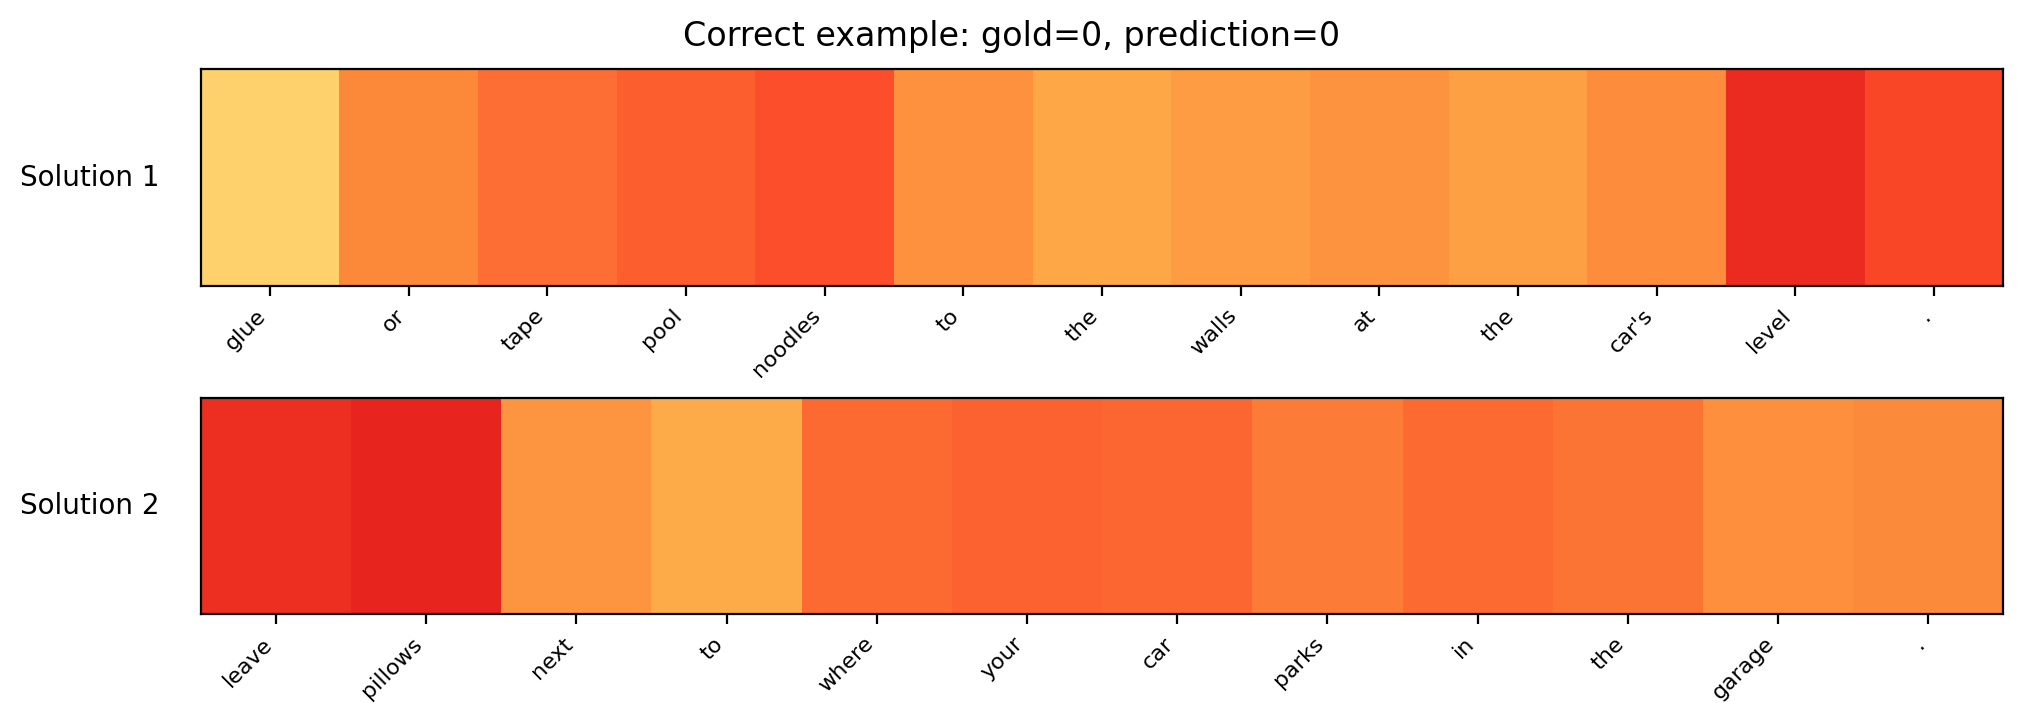
\includegraphics[width=0.49\textwidth]{attention_correct.png}\hfill
  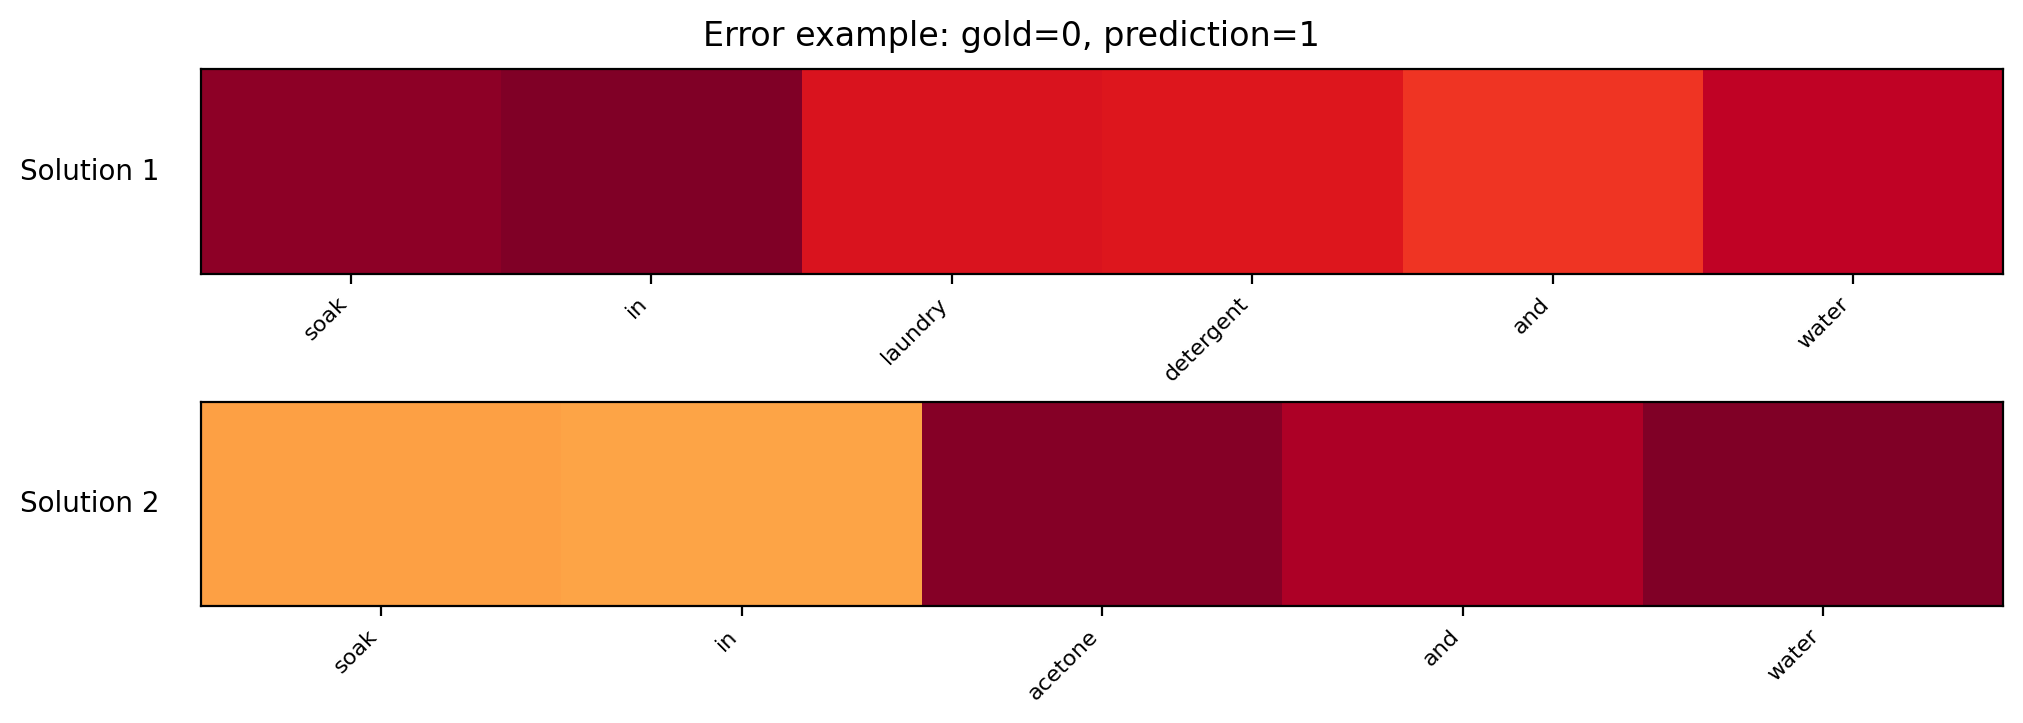
\includegraphics[width=0.49\textwidth]{attention_error.png}
  \caption{Goal-conditioned attention for a correct car-protection case (left) and an incorrect shoelace-cleaning case (right). Darker cells have greater weight; each row is normalised independently.}
  \label{fig:attention}
\end{figure*}

\section{Conclusion}
We presented a reproducible, from-scratch PIQA system that combines a shared BiGRU, goal-conditioned attention, explicit goal--candidate interactions, and swap-equivariant pair contrast. Its $60.65\pm0.33$ test accuracy exceeds three group-run baselines, and controlled ablations identify contrast as the most useful design choice. The gains are nevertheless small and early overfitting plus the acetone failure expose a central limitation: distributional text supervision alone provides weak grounding for physical consequences. Future work could regularise attention, test character/subword encoders for rare objects, and use auxiliary objectives derived strictly from the supplied training pairs; pretrained or multimodal baselines would also contextualise the scratch-model ceiling if compute permits.

\clearpage
\section*{Team Contributions}
\textbf{Replace before submission.} Group member names and their specific contributions were not supplied with the assignment files. For an individual submission, replace this paragraph with: ``This project was completed individually; all design, implementation, experiments, analysis, and writing were undertaken by [name].'' For a group, list each member and a concise description of their contribution.

\bibliography{references}

\end{document}
